%%%%%%%%%%%%%%%%%%%% author.tex %%%%%%%%%%%%%%%%%%%%%%%%%%%%%%%%%%%
%
% sample root file for your "contribution" to a contributed volume
%
% Use this file as a template for your own input.
%
%%%%%%%%%%%%%%%% Springer %%%%%%%%%%%%%%%%%%%%%%%%%%%%%%%%%%


% RECOMMENDED %%%%%%%%%%%%%%%%%%%%%%%%%%%%%%%%%%%%%%%%%%%%%%%%%%%
\documentclass[graybox]{svmult}

% choose options for [] as required from the list
% in the Reference Guide

\usepackage{mathptmx}       % selects Times Roman as basic font
\usepackage{helvet}         % selects Helvetica as sans-serif font
\usepackage{courier}        % selects Courier as typewriter font
\usepackage{type1cm}        % activate if the above 3 fonts are
                            % not available on your system
%
\usepackage{makeidx}         % allows index generation
\usepackage{url}             % links
\usepackage{graphicx}        % standard LaTeX graphics tool
                             % when including figure files
\usepackage{multicol}        % used for the two-column index
\usepackage[bottom]{footmisc}% places footnotes at page bottom

\usepackage{algorithm}
\usepackage[noend]{algpseudocode}

% see the list of further useful packages
% in the Reference Guide

\makeindex             % used for the subject index
                       % please use the style svind.ist with
                       % your makeindex program

%%%%%%%%%%%%%%%%%%%%%%%%%%%%%%%%%%%%%%%%%%%%%%%%%%%%%%%%%%%%%%%%%%%%%%%%%%%%%%%%%%%%%%%%%

\begin{document}

\title*{Accelerated Load Balancing of Unstructured Meshes}
% Use \titlerunning{Short Title} for an abbreviated version of
% your contribution title if the original one is too long
\author{
Gerrett Diamond,
Lucas Davis,
Cameron W. Smith,
and Mark S. Shephard
}
\institute{
  Gerrett Diamond \email{diamog@rpi.edu}
  \and Lucas Davis \email{davisl3@rpi.edu}
  \and Cameron W. Smith \email{smithc11@rpi.edu}
  \and Mark S. Shephard \email{shephard@rpi.edu}
  \at Rensselaer Polytechnic Institute, Troy, NY 
}
\authorrunning{G.Diamond et al.}

\maketitle

\abstract{
  In order to take advantage of distributed systems it is necessary to parallelize as many steps as possible in a work flow. Adaptive meshes often need load balancing to properly utilize the available concurrent computing resources. By representing the mesh as a hypergraph and utilizing coloring algorithms a desirable geometric partitioning can be achieved. By taking advantage of parallel architecture throughout the cost the process of creating a hypergraph and coloring is less than a typical geometric partitioning.
}

\section{Introduction} \label{sec:intro}

%\begin{itemize}
%  \item briefly motivate dynamic load balancing
%  \item quantify how GPUs are providing the majority of computing performance (\# of systems with GPUs in top 10 systems of top500, graph500, HPCG)
%  \item end with a sentence that says what engpar does (diffusion) and how we are
%extending it to run on GPUs
%\end{itemize}

Unstructured mesh applications running on current and next generation machines require the
computational work related to mesh entities to be evenly distruibuted across processes in
order to achieve maximal performance. While common partitioning techniques such as multilevel
[REFERENCES] or geometric [REFERENCES] methods are good for creating an initial distribution
of load, evolving simulations where the mesh and computational load changes during the
simulation require dynamic load balancing techniques that are quick to improve the partition
as the work load changes. Diffusive load balancing methods allow quick partition refinement
for the relatively small changes to imbalance that are seen in adaptive mesh simulations.

\section{EnGPar Dynamic Load Balancing} \label{sec:engpar}

%\begin{itemize}
%  \item multi-graph, high-level diffusion algorithm (targeting, selection, migration)
%  \item indicate that we will accelerate selection via BFS for distance computation and coloring for cavity selection
%\end{itemize}

EnGPar is a partition improvement tool that utilizes a specialized multi-hypergraph,
called the N-graph, to describe the portions of the mesh that require load balancing.
The N-graph consists of vertices which represent the primary dimension entities of the
mesh. The vertices are connected by hyperedges created from the secondary dimensions of
the mesh that require load balancing. Figure \ref{fig:ngraph} shows the conversion from
mesh (a) to hypergraph (b) where mesh faces are used to create the graph vertices and
mesh vertices are represented by hyperedges. A second edge type is used to represent mesh edges in (c). 

\begin{figure}[!ht]
  \centering
  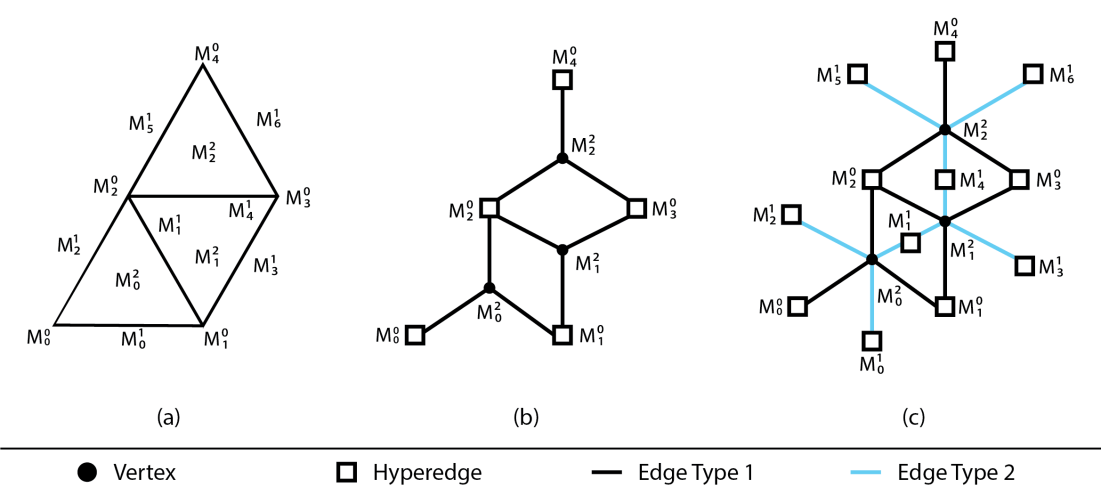
\includegraphics[width=3.5in]{images/exampleMesh2Graph.png}
  \caption{A triangular mesh (a) converted to the N-graph with mesh faces represented by graph vertices and mesh vertices as hyperedges (b) and mesh edges as a second hyperedge type (c).}
  \label{fig:ngraph}
\end{figure}

EnGPar's diffusive algorithm is an iterative local refinement strategy where in each
iteration the target criteria is improved until the imbalance is under a given
tolerance or the imbalance cannot be improved further. Each iteration consists of three
steps: targeting, selection, and migration.
Algorithm~\ref{alg:engpar} lists the pseudo code.
The targeting phase consists of gathering
metrics on the part and its neighbors in order to determine which neighboring parts to
send weight to and how much weight to send. The selection step is where graph vertices
on the boundary are chosen to be sent to neighboring parts in order to satisfy the
weights determined by the targeting phase. Finally, the migration phase sends the graph
entities that were selected to the destination parts and the graph is reconstructed.

\begin{algorithm}[H]
  \caption{Diffusive Load Balancing Framework}
  \label{alg:engpar}
  \small
  \begin{algorithmic}[1]
    \Procedure{Balance}{$ngraph$,$entity\_types$}
    \ForAll{$t \in entity\_types$}
    \While{imbalance of $t >$ tolerance}
    \Call{RunStep}{$ngraph$,$t$}
    \If{Balancing Stagnates}
    \State break
    \EndIf
    \EndWhile
    \EndFor
    \EndProcedure

    \Procedure{RunStep}{$ngraph$,$t$}
    \State $sides = makeSides(ngraph)$
    \State $weights = makeWeights(ngraph,sides,t)$
    \State $targets = makeTargets(ngraph,sides,weights)$
    \State $queue = makeQueue(ngraph)$
    \State $plan = select(ngraph,targets,queue)$
    \State $ngraph.migrate(plan)$
    \EndProcedure
  \end{algorithmic}
\end{algorithm}

In this work, we target accelerating distance computation and cavity selection.
%This estimate is high as the timings for the 'planning' includes some
%communication and the trim procedures that will not be accelerated in this
%work.  Timings show that distance computation takes between 5\% and 16\% of the
%total time.  Need to re-run with selection timers.
As shown by the `Balancing' bar in Figure~\ref{fig:partsgraph}, these two
procedures consume up to 50\% of the total execution time and are well suited to
acceleration as they do not require communications~\cite{engparSC17}.

\begin{figure}
  \centering
  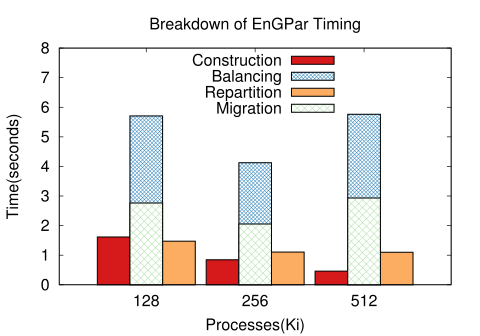
\includegraphics[width=3in]{images/timeparts_v_cores.png}
  \caption{A breakdown of timing for each step of the EnGPar runs. The
    bottom part of the bar for balancing represents the migration
    component of the balancer.~\cite{engparSC17}}
  \label{fig:partsgraph}
\end{figure}

Distance computation is performed by the $makeQueue$ function of
Algorithm~\ref{alg:engpar} where hyperedges on the boundary are ordered based on
their distance from the center of the part from furthest to closest.
EnGPar computes this distance with two breadth first traversals of the graph.
Figure~\ref{fig:distQueue} depicts the topological distances on a single part of
a 2D triangular mesh.
The vertices in the left side of Figure~\ref{fig:distQueue} are labelled with
the topological distance from the part boundary that results from the first
traversal from the outside-in.
The right side shows the distance from one of the deepest vertices (distance
three) to the part boundary that results from the second traversal from the
inside-out.

\begin{figure}
  \centering
  \label{fig:distQueue}
  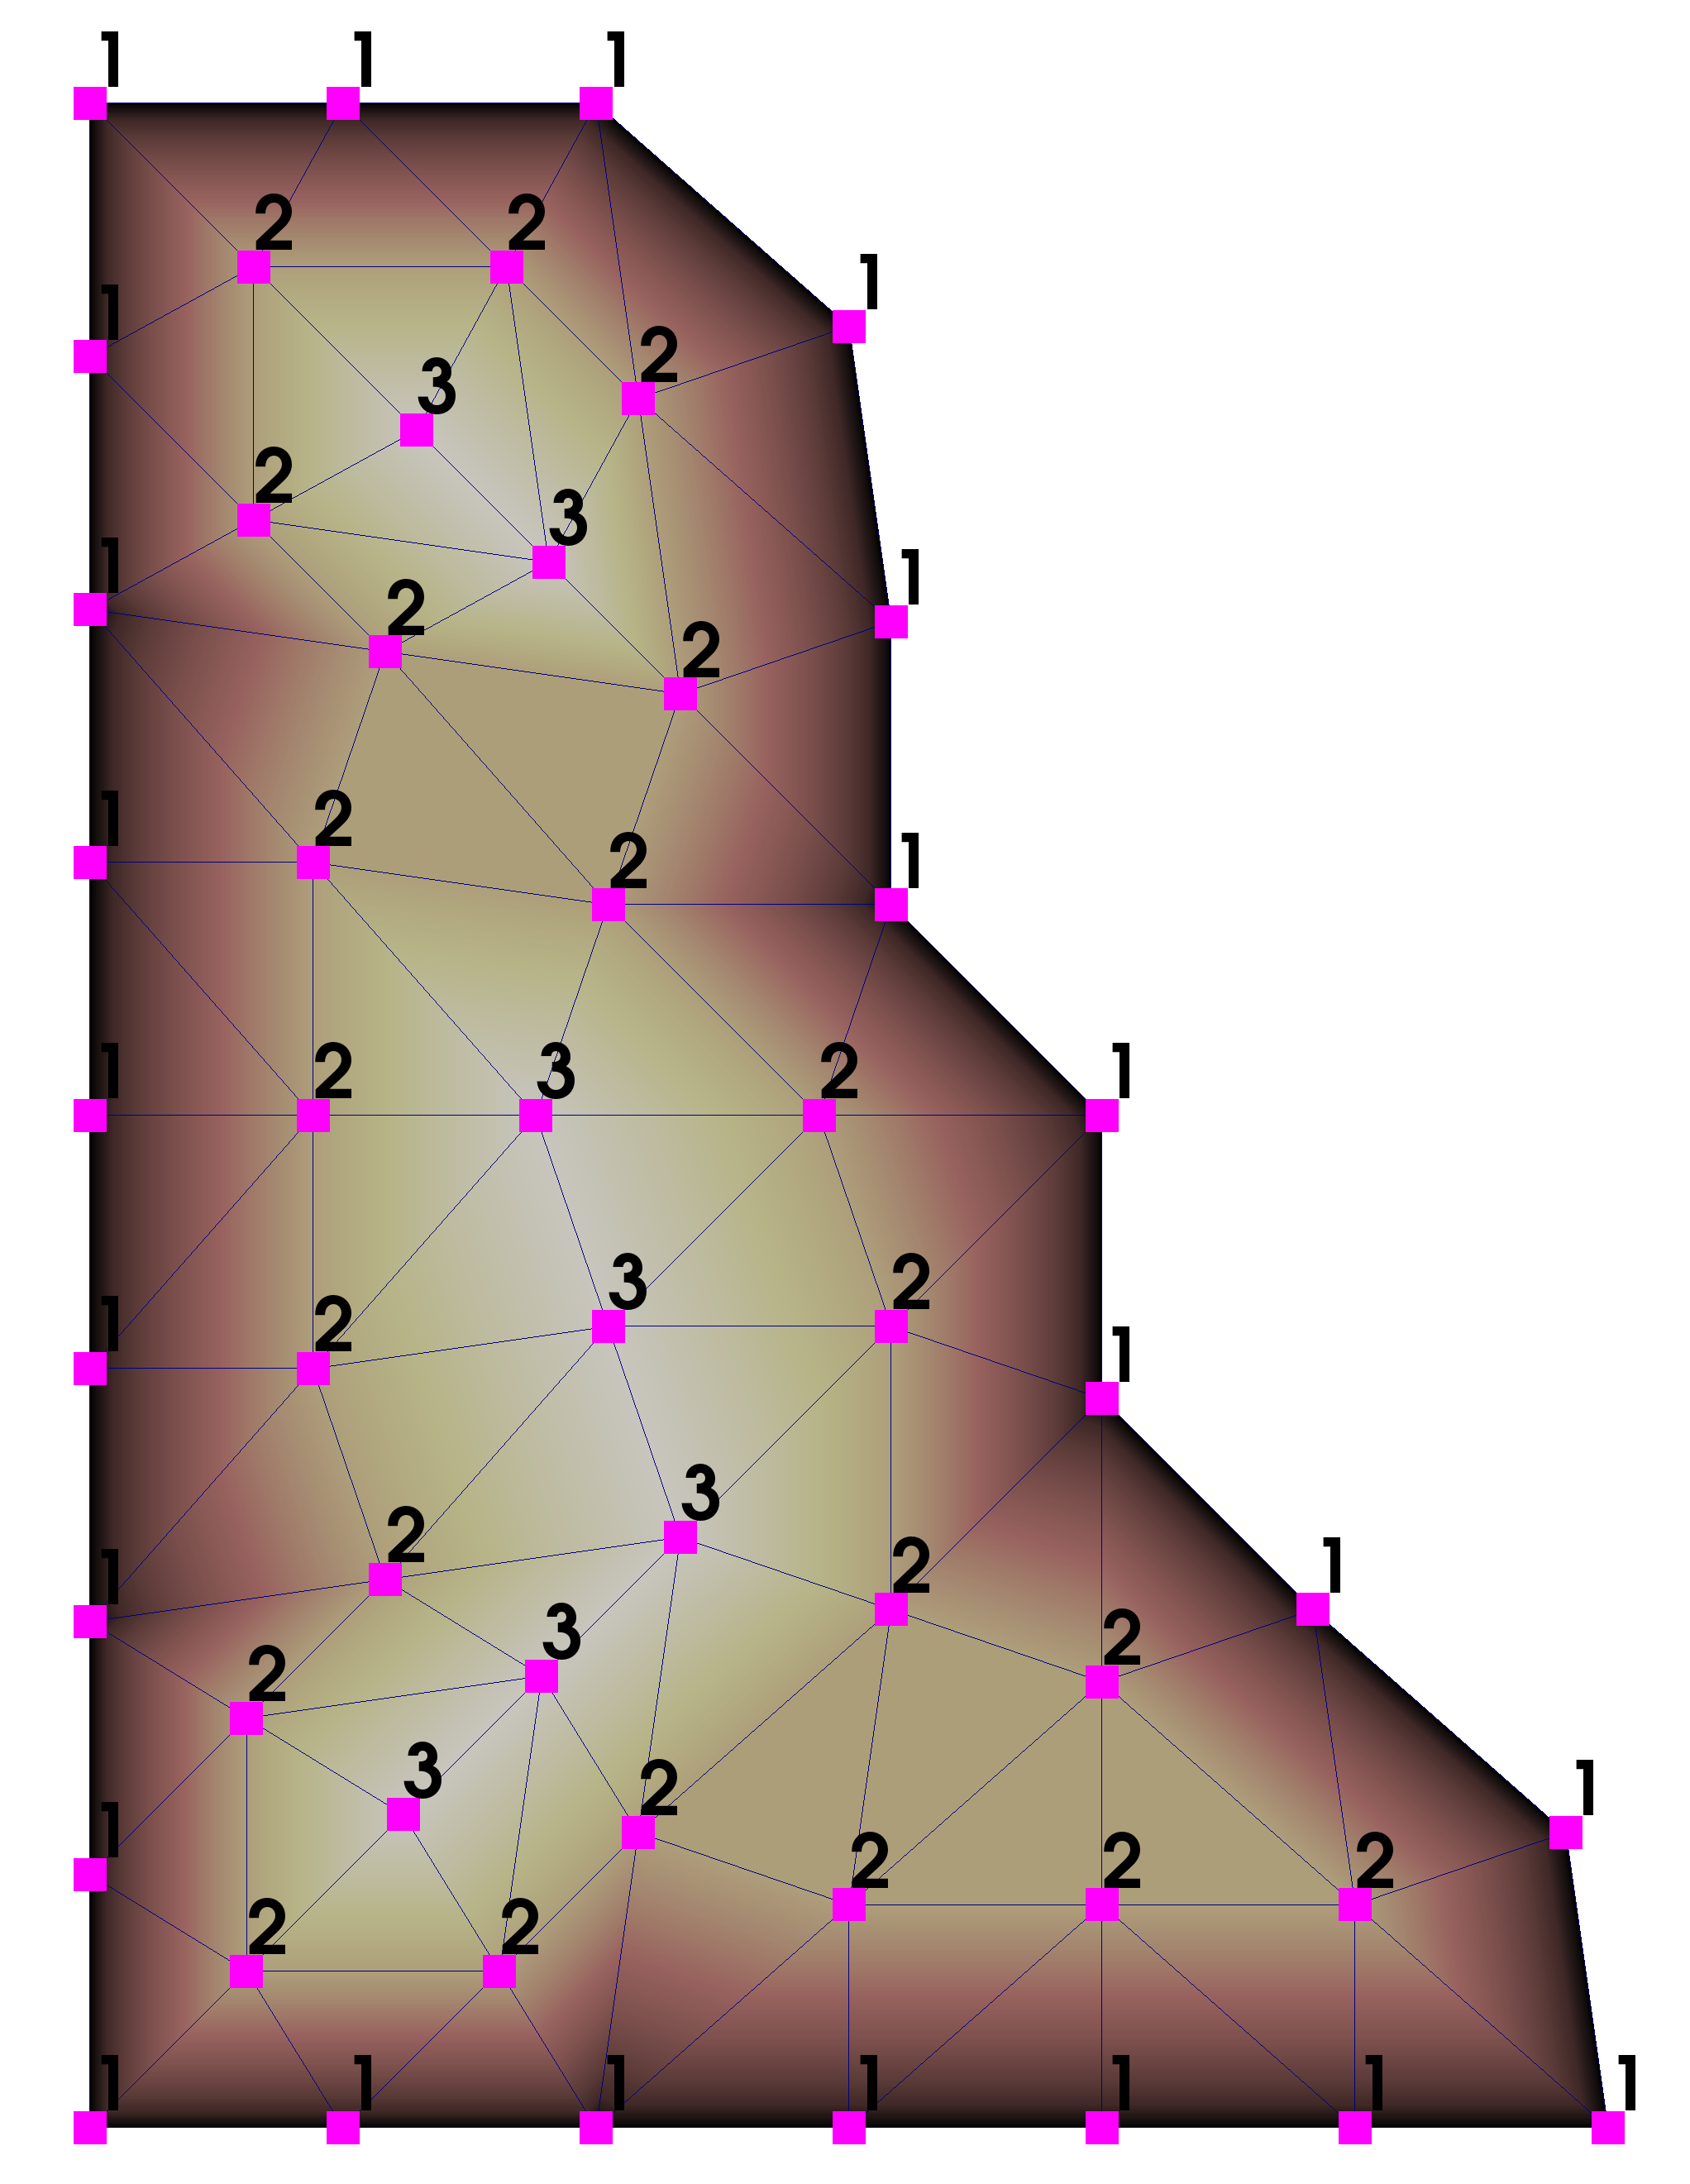
\includegraphics[width=.4\textwidth]{images/2dTreeDepth.png}
  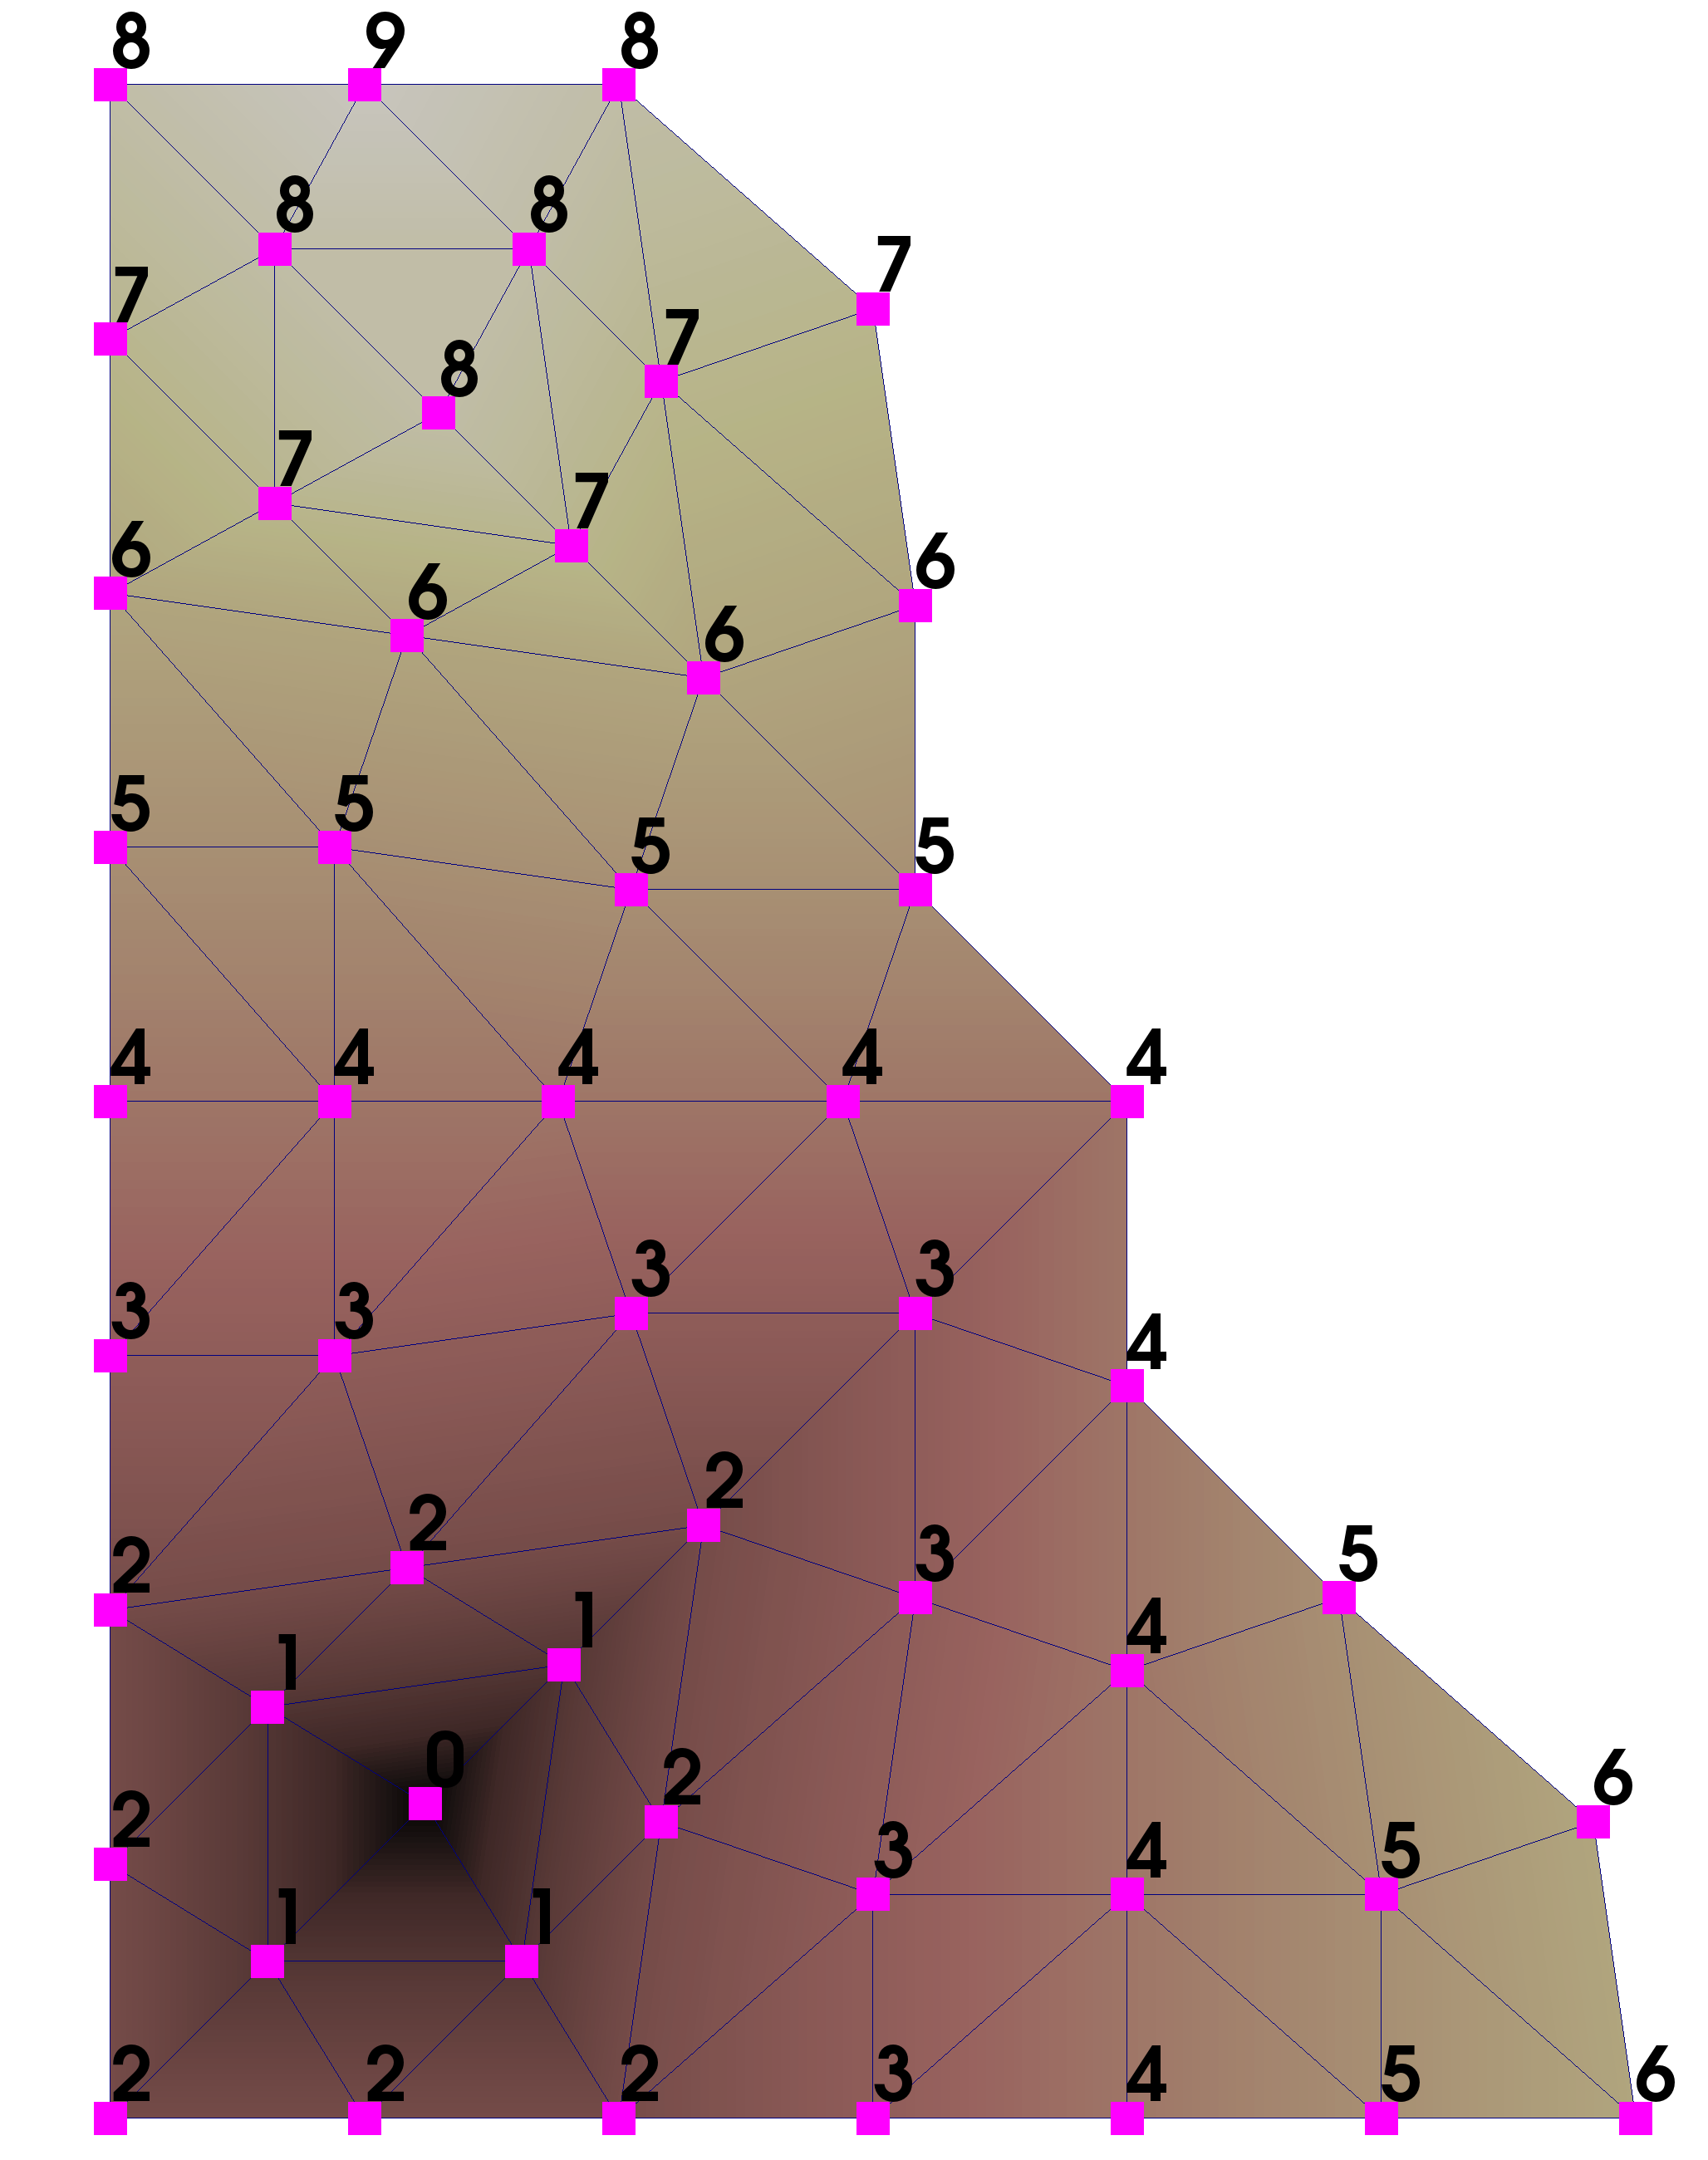
\includegraphics[width=.41\textwidth]{images/2dDistance.png}
  \caption{
    (left) The distance from each vertex to the boundary and (right) the
    distance from the core vertex (marked with a zero near the
    bottom left corner).~\cite{SmithParma2015}
  }
\end{figure}

Cavity selection, the $select$ function of Algorithm~\ref{alg:engpar},
determines if a cavity, defined as a hyperedge and the vertices that are
connected by it, on the part boundary should be sent to neighboring parts.
Figure~\ref{fig:partBdry} depicts two cavities on the part boundary being
evaluated for migration from part 0 (bottom) to part 1 (top).
A cavity is selected for migration if (1) the part that the hyperedge is shared
with is a target part, (2) the target part has not been sent more weight than
the limit, and (3) the size of the cavity is small.

\begin{figure}
  \label{fig:partBdry}
  \centering
  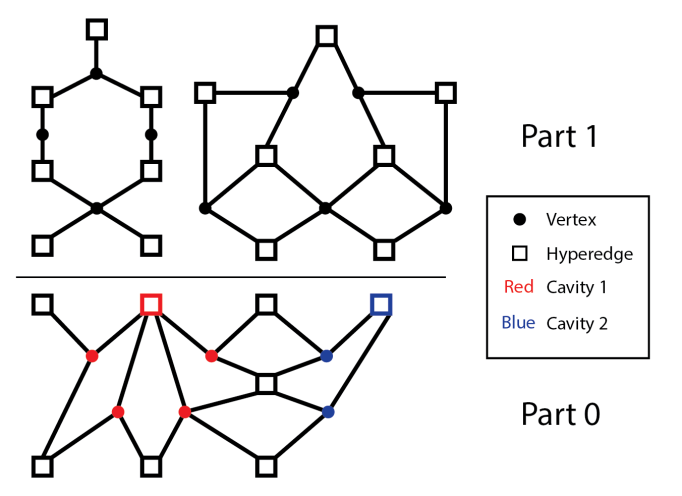
\includegraphics[width=0.8\textwidth]{images/PartBoundary.png}
  \caption{Two parts of an N-graph sharing four hyperedges at the part boundary.
    Two of the four cavities formed from the hyperedges on part 0 are shown in
    red and blue.
  }
\end{figure}

\section{Accelerating Distance Computation} \label{sec:dist}

Distance computation's breadth first traversal is accelerated with a OpenCL
data-parallel ND-Range kernel for execution on GPUs and many-core processors.
The host process calls the kernel once for each frontier in the traversal.
The kernel implementation iterates over the graph vertices
pinned to each hyperedge twice.
The first iteration determines if in the previous iteration any vertices were
marked with a distance equal to the current frontier depth.
If a vertex is found then the second iteration updates the distance of the other
vertices.
This `pull' based-implementation is well explored in literature REFERENCES.

The OpenCL pull implementation executes on a compressed sparse row (CSR) hypergraph
representation and is compared to additional implementations that
optimize the data structure and loops for uniform hypergraph-to-vertex
connectivity.
When the hypergraph is constructed from a unstructured mesh of tetrahedron, such
that mesh vertices map to graph vertices and mesh elements to
hyperedges, the number of vertices pinned to each hyperedge is exactly four.
The uniform structure is leveraged by an implementation using the Sell-C-Sigma
BESTA-and-MERENDING and manual hyperedge-to-vertex loop unrolling.
In addition to these variants performance comparison is also provided for
implementations using four byte integers, instead of eight byte, and a serial
C++ `push` implementation.

Figure~\ref{fig:bfs} depicts the performance of the different implementations
relative to the `csr' implementation using the pull approach and a CSR
hypergraph data structure.
`scg' in the name of the implementation indicates that use of the Sell-C-Sigma
data structure, `int' indicates use of four byte integers, and `unroll'
indicates manual vertex loop unrolling.
Runs were executed on the graphs listed in Table~\ref{tbl:uprightCounts} created
from meshes of the 2014 RPI Formula Hybrid suspension upright depicted in
Figure~\ref{fig:upright}.
All tests were executed on an NVIDIA 1080ti using CUDA 9.2 (driver 396.26) on
RedHat7 with GCC 4.8.5.
The chunk size of the `scg' tests was fixed at 64; given the uniform degree of
the test meshes there was no appreciable performance difference between
different chunk size settings.
Reported timings are the average of three runs.
Timings include data transfers to and from the GPU.
The OpenCL JIT compilation time is not included in the timing as this one-time
cost would be amortized across tens of diffusive iterations.

\begin{figure}
  \begin{minipage}{0.4\textwidth}
    \label{fig:upright}
    \centering
    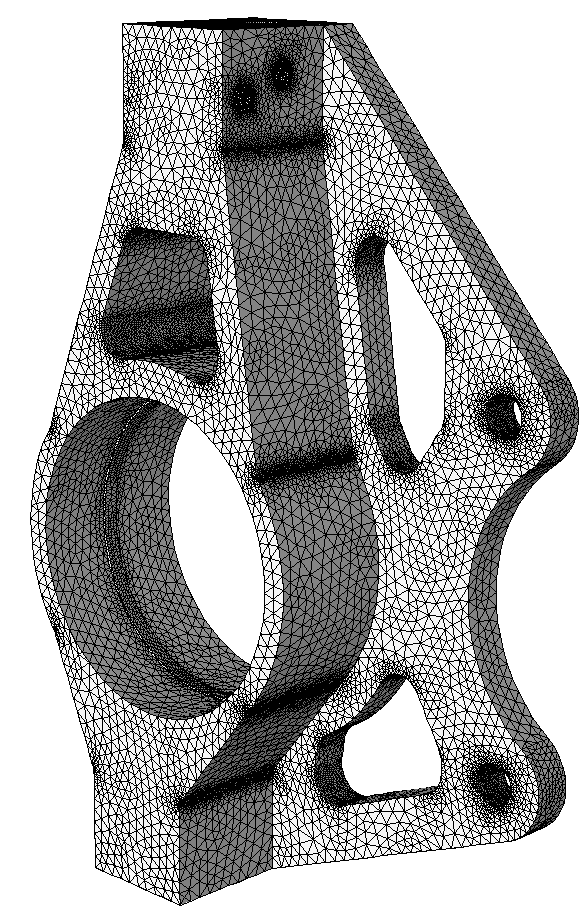
\includegraphics[width=.4\textwidth]{images/upright400k.png}
    \caption{400k element mesh of the 2014 RPI Formula Hybrid suspension upright.}
  \end{minipage}\hfill
  \begin{minipage}{0.5\textwidth}
    \label{tbl:uprightCounts}
    \begin{tabular}{l|rrrr}
      graph & vertices & hyperedges & bfs levels & max frontier  \\
      \hline
      67k   & 66433    & 15697      & 25         & 4432          \\
      190k  & 192728   & 40052      & 40         & 7992          \\
      400k  & 404613   & 88651      & 48         & 17316         \\
      890k  & 890925   & 187380     & 70         & 26664         \\
      1.6M  & 1580611  & 336215     & 82         & 45268         \\
      13M   & 12831104 & 2499193    & 82         & 95798         \\
      28M   & 27943315 & 5190006    & 210        & 128035
    \end{tabular}
    \caption{Hypergraphs created from upright meshes. The suffix 'k' is shorthand
    for thousand and 'M' is for million.}
  \end{minipage}
\end{figure}

\begin{figure}
  \centering
  \label{fig:bfs}
  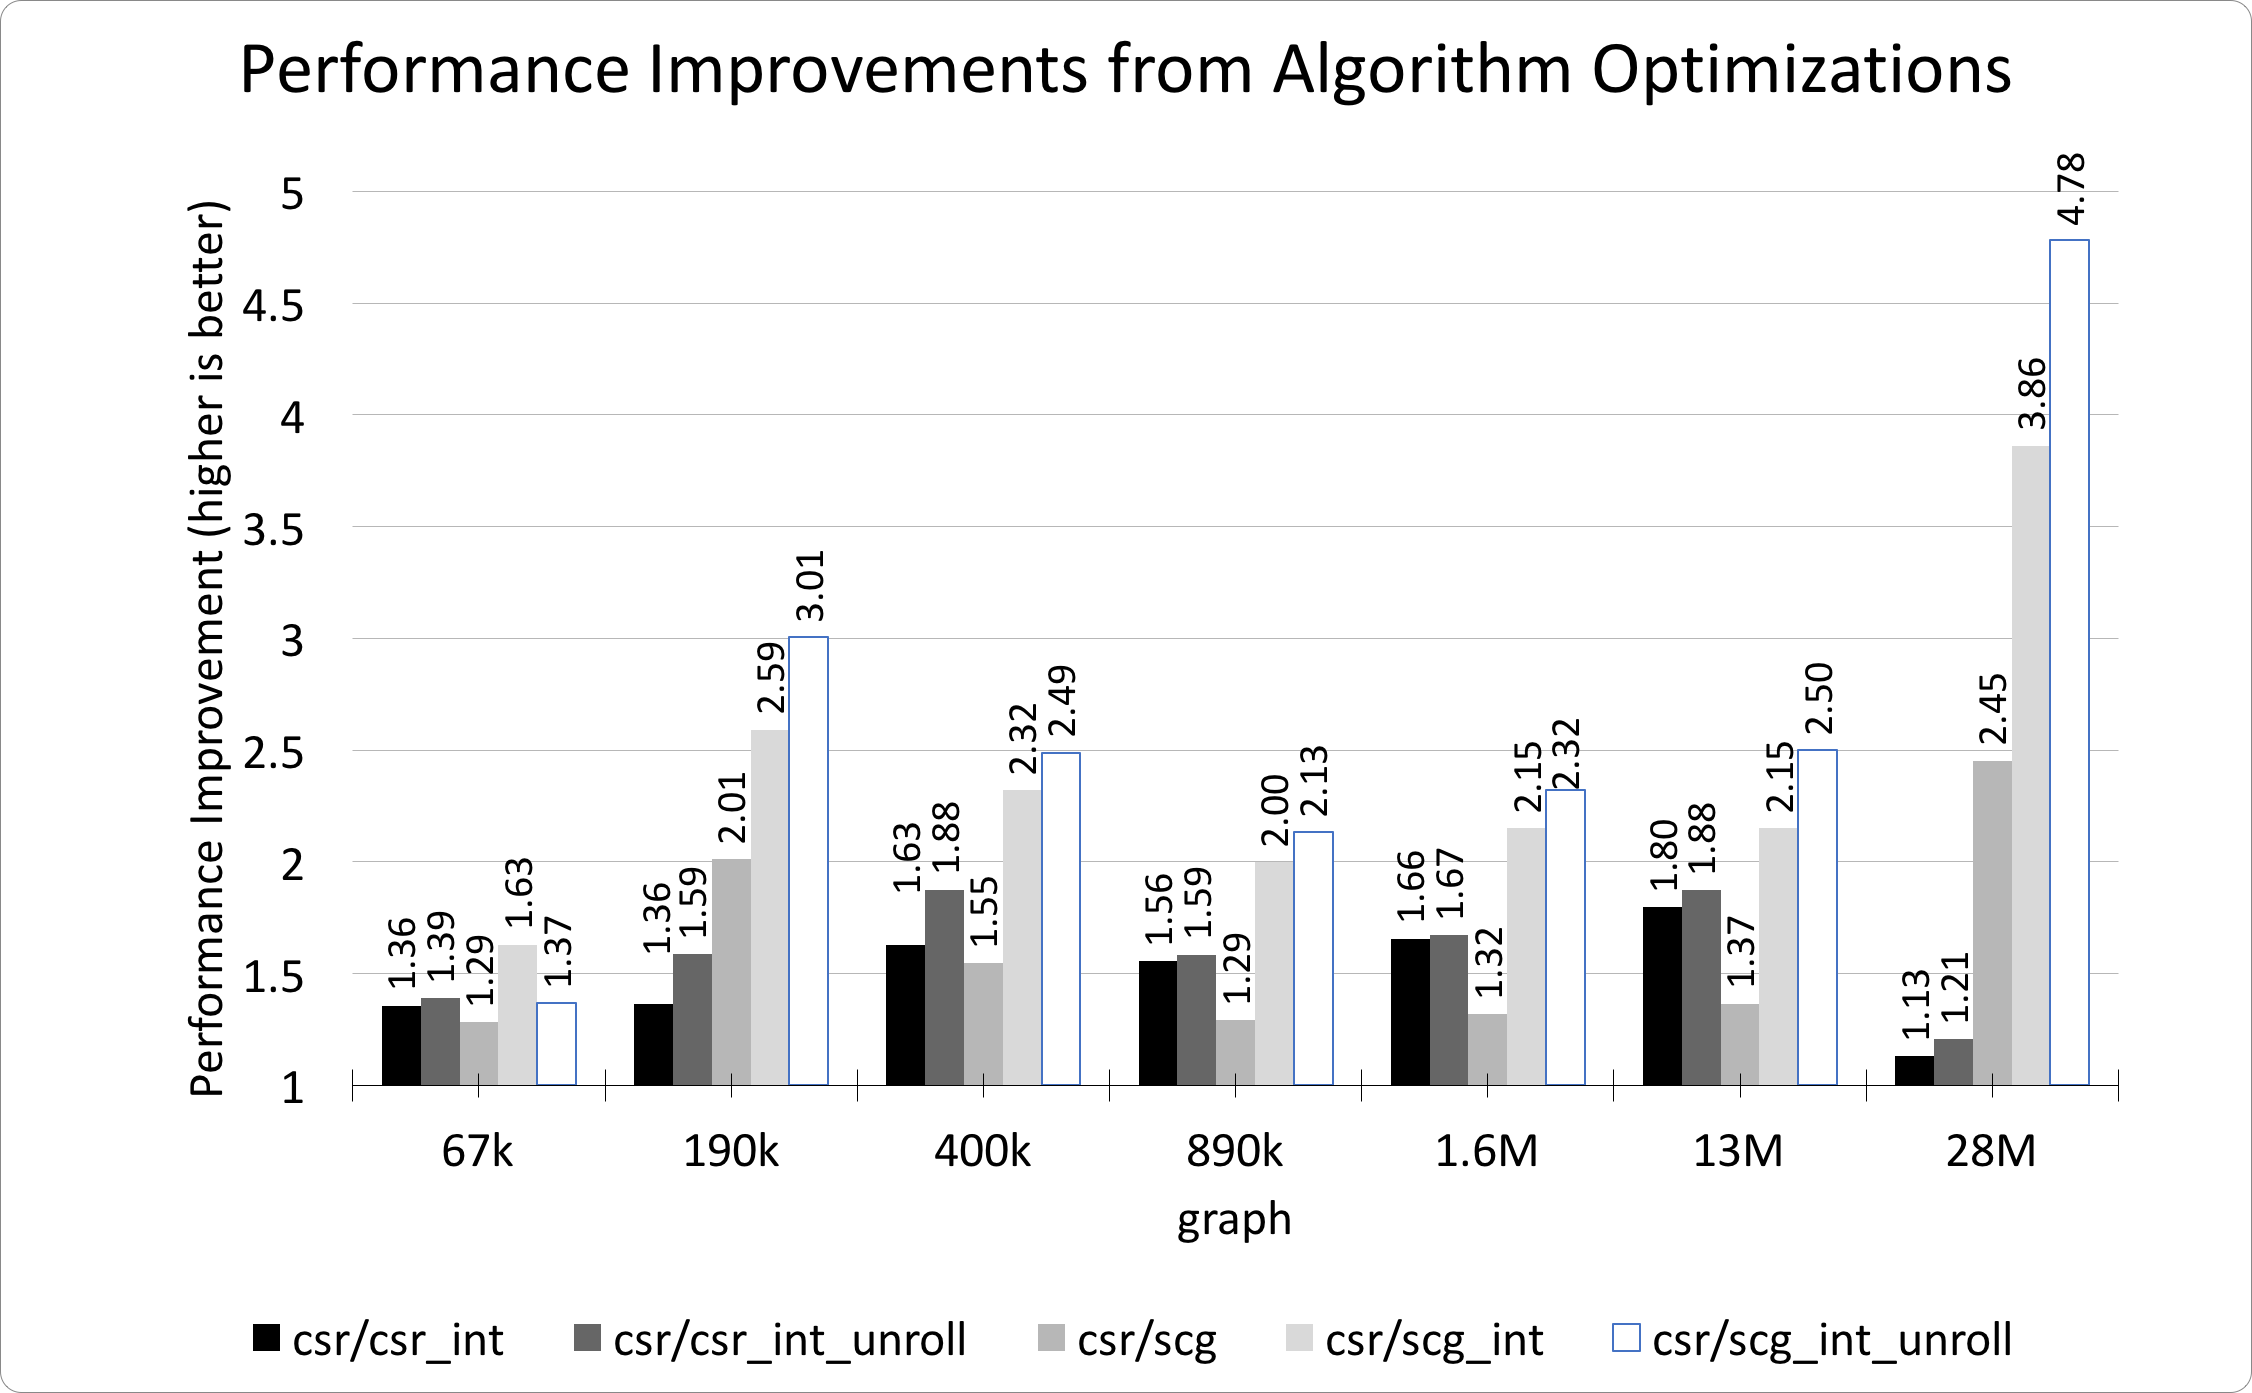
\includegraphics[width=0.8\textwidth]{images/bfsPerformance.png}
  \caption{
    Performance of various breadth first traversal OpenCL data-parallel implementations
    relative to the baseline `csr' implementation.
  }
\end{figure}

On the largest mesh with 28 million elements, the `scg\_int\_unroll' is 11 times
faster than the serial C++ push based implementation and 4.78 times faster than
the `csr' implementation.
The performance boost given by loop unrolling and use of the Sell-C-Sigma data
structure are the result of improved memory coalesing.
Reducing the integer size by half improves performance by 24\% for the 28
million element mesh.

\section{Accelerating Cavity Selection} \label{sec:select}

Accelerating the selection of cavities requires simulateously evaluating many
cavities.
The current single threaded selection procedure evaluates cavities in order of
their descending distance from the topological center.
Since the ordered selection exposes no concurrency an alternative application of
the topological distance is needed.
One approach is to bin the cavities by distance.
For large parts, or parts with high surface area, this will expose a modest
amount of concurrency.
A second approach applies the topological distance sorting after a fully
parallel cavity evaluation has executed.
Given that this approach provides maximum concurrency during cavity evaluation,
and can use a data-parallel sorting operation, it is the procedure guiding this
work.

Critical to concurrent cavity evaluation is avoiding race conditions when
writing and reading the integer associated with each graph vertex indicating
which process they will be migrated to.
Hyperedge coloring ensures that any two hyperedges that share a common vertex
will be assigned a different color.
Hyperedges with the same color can be evaluated concurrently without
race conditions.
In Figure~\ref{fig:partBdry}, the red and blue colored cavities do not share any
vertices and thus could be processed simultaneously.

The Kokkos-kernels data-parallel graph coloring procedure~\cite{kokkosColoring} is used to
color the hyperedges of the EnGPar hypergraph.
This procedure is driven by a symmetrix adjacency matrix.
To color hyperedges that don't share vertices we must create the
hyperedge-to-vertex-to-hyperedge adjacency matrix (herein referred to as `EVE');
the dual of the hypergraph.
The EVE graph has one vertex for each hyperedge, and an edge between two
hyperedges if they share at least one common vertex.
Kokkos-kernel's graph coloring algorithm is then called to color this dual graph
which returns a coloring of the original graph's hyperedges.

\subsubsection{Parallel EVE Construction}

The construction of the second adjacency crs matrix starts by making a
set that stores hyperedge-to-hyperedge adjacencies. Because the information being read and written should not overlap or change due to race conditions parallelism can be leveraged to improve performance. Using the map two single dimension arrays, \verb|deg| and \verb|edgeList|, are created to represent the graph. Because \verb|deg| stores degree of each edge, a parallel reduction is utilized to find the total degree of an edge then a parallel prefix sum modifies the \verb|deg| array to store the total number of entries up to row \verb|i| exclusively. \verb|edgeList| stores the column index of the non-zero matrix entries which are the hyperedge labels in this construction. The column index in this case represents the edge adjacent to the edge labeled by the row index.

\begin{algorithm}[H]
\caption{Dual Graph Converter}
\label{alg:dual}
\algloopdefx[PFor]{PFor}[1]{\textbf{parallel for} #1 \textbf{do}}
\algblock[Name]{Start}{End}
\algblockdefx[NAME]{START}{END}
  [1][a]{\textbf{parallel for} #1 \textbf{do}}
\small
\begin{algorithmic}[1]
\Procedure{CREATE DUAL CSR}{$G=(V,E)$}
  \State $n = 0$
  \PFor{$v \in V$}
    \ForAll{$(i,v) \in E$}
      \ForAll{$(j,v) \in E\setminus\{(i,v)\}$}
        \State $n$++
      \EndFor
    \EndFor
  \State set of int pair $m$ (n) \Comment{n is a upper bound on the set's size}
  \PFor{$v \in V$}
    \ForAll{$(i,v) \in E$}
      \ForAll{$(j,v) \in E\setminus\{(i,v)\}$}
        \State m.insert ( $(i,j)$ )
      \EndFor
    \EndFor
  \State $N=|E|$
  \State deg = [$N+1$]
  \PFor {$k\in m$}
    \State deg($k$.first+1)++
  \PFor{$i=0,1,\ldots,N$}
    \State deg[$i$] = sum(deg[$0:i$])
  \State edgeList = [deg[N]]
  \State degreeCount = [N]
  %\PFor {$k\in m$}
  \START[$k\in m$]
  	\State e = deg[k.first] 
    \State i = degreeCount[k.first]++
  	\State edgeList[e+i] = k.second
  \END
  \EndProcedure
\end{algorithmic}
\end{algorithm}
This algorithm converts a hypergrpah to its dual. The number of adjacencies are counted then used to initialize the set to avoid needing to allocate more memory later in the algorithm. Two arrays are created to store the graph information, deg and edgeList. These store the offset of a vertex into the list of vertices adjacent to it. The construction is able to take advantage of parallelism to parse the graph and write the arrays. Together the two arrays represent the graph in compressed sparse row format which can be passed directly to a parallel graph coloring algorithm. This coloring algorithm is implemented in Kokkos Kernels \textbf{REFERENCE}.

\section{Application Results} \label{sec:results}

% TIMING RESULTS
\begin{figure}[!ht]
	\centering
	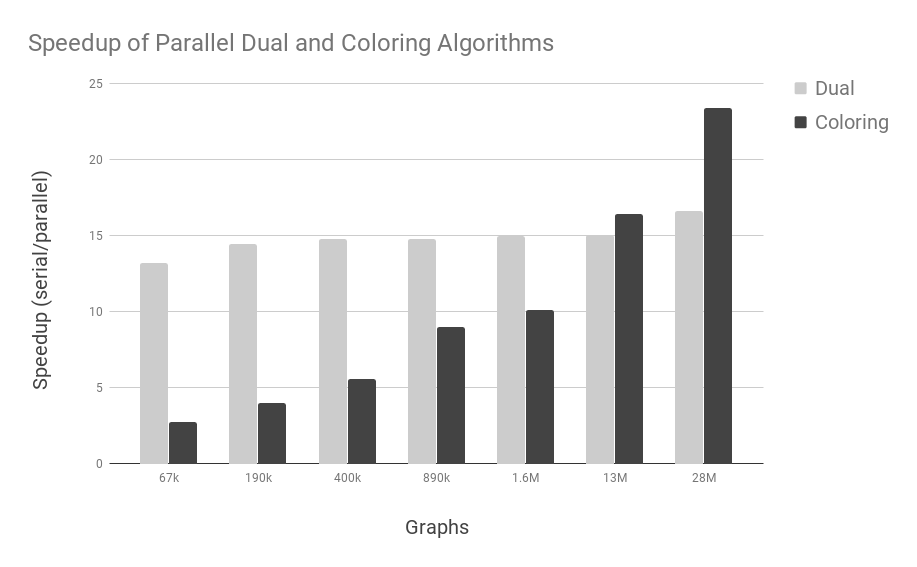
\includegraphics[width=4in]{images/Parallel_Speedup.png}
	\caption{The ratio of serial execution time to parallel for dual graph construction and graph coloring}
	\label{fig:coloringSpeedup}
\end{figure}
The timing speedup results shown in \textbf{Fig. 2} demonstrate that parallelism speeds up both coloring and dual graph construction. The compiler used was gcc 4.8.5 with compiler flags -O2 on a redhat 7 OS with a GeForce GTX 1080 Ti running nvidia 396.26 and cuda version 9.2. It is notable that the speedup to graph construction is nearly constant while the increase to graph coloring continues to grow with the problem size.

%\begin{itemize}
%  \item Figure out a better title for this section
%  \item flow control strong scaling case with 1.3B tets: \\
%64Ki \url{https://zenodo.org/record/833519#.WztuxXWYV1M} \\
%128Ki \url{https://zenodo.org/record/834946#.Wztu-HWYV1M} \\
%256Ki \url{https://zenodo.org/record/835483#.WztvCXWYV1M} \\
%512Ki \url{https://zenodo.org/record/835742#.WztvG3WYV1M}
%  \item the number of elements per-process may be too small for nodes with large GPUs to run efficiently (data transfer may become more costly than running the selection on the CPU!) - especially as we approach 512Ki parts
%  \item we will have to run the condense tool to create an 2Ki (640k elms/part),
%    4Ki (320k), 8Ki (160k), 16Ki (80k), and 32Ki (40k) meshes -
%    fun3d uses between 75M and 2.3M elements per GPU on summitdev (from siampp18
%    presentation)
%  \item run on ORNL titan or summit (if accessible)
%  \item compare runtimes versus results from SC17 paper~\cite{engparSC17}
%  \item use mesh vertex = graph vertex and mesh edge = graph edge for tests -
%    will need to run MPI only engpar to establish the baseline performance
%  \item plot the time spent in MPI only selection vs kokkos coloring selection
%    vs part size - the comparison must start and end at equivalent points in the
%    code - start before selection and end just before migration (or whatever the
%    next stage) begins
%  \item plot the breakdown of time spent in coloring selection vs part size -
%    data transfer, color computation, selection (possibly broken into cavity
%    selection and filtering for distance), tranferring the selection list
%    back to the host
%  \item I expect there will be some reduction in partition quality using the
%    coloring based selection since we won't have as fine-grained control over
%    the process as the MPI only procedure.  As long as the quality reduction is
%    controlled and performance is better we should be OK.
%\end{itemize}

\section{Closing Remarks} \label{sec:closing}
\begin{itemize}
  \item summarize results
  \item discuss hypergraph coloring and relation to distance-2 coloring for non-simplices (quads, hexs, prisms, pyramids, etc.)
\end{itemize}

\begin{acknowledgement}
This research was supported by the U.S. Department of Energy, Office of Science,
Office of Advanced Scientific Computing Research, under award DE-SC00066117
(FASTMath SciDAC Institute) and by the National Science Foundation under Grant
No. ACI 1533581, (SI2-SSE: Fast Dynamic Load Balancing Tools for Extreme Scale
Systems).
Any opinions, findings, and conclusions or recommendations expressed in this
material are those of the author(s) and do not necessarily reflect the views
of the National Science Foundation.
\end{acknowledgement}

\bibliographystyle{acm}
\bibliography{scorec-refs/scorec-refs}
\end{document}
